\section{S1 -- Tryby komunikacji między procesami w standardzie Message Passing Interface}

\textbf{MPI} stanowi standard przesyłania komunikatów pomiędzy procesami programów równoległych działających na jednym lub więcej komputerach. Pracuje natywnie z C, C++, Fortranem. Istnieją rozwiązania dla innych języków np. Python, lecz stanowią tylko nakładki na wyżej wymienione. Dostępne wersje biblioteki:
\begin{itemize}
\item Wersja 1.2 (MPI-1) -– wprowadza około 150 funkcji;
\item Wersja 2.1 (MPI-2) -– rozszerzona o nową funkcjonalność, razem ponad 500 funkcji
\end{itemize}

Standard/biblioteka występują w wielu implementacjach. Najpopularniejsze z nich to:  MPICH / MPICH2, OpenMPI, Intel MPI, HP MPI. 

Informacje podstawowe: 
\begin{itemize}
\item program lub jego części mogą wykonywać się jednocześnie na więcej niż jednej jednostce obliczeniowej;
\item jednostka obliczeniowa: procesor, rdzeń procesora, wątek sprzętowy, wątek systemowy, inne;
\item \textbf{Komunikatorem} nazywam zbiór procesów mogących się wzajemnie komunikować;
\begin{itemize}
\item \texttt{\textbf{MPI\_Comm\_size}(MPI\_COMM\_WORLD, \&np)} – zwraca listę procesów wewnątrz komunikatora;
\end{itemize}
\item Tak samo jak w przypadku procesów w systemie operacyjnym wewnątrz komunikatora każdy proces otrzymuje unikalny identyfikator (numer) tzw. \textbf{rank};
\begin{itemize}
\item \texttt{\textbf{MPI\_Comm\_rank}(MPI\_COMM\_WORLD, \&rank)} – zwraca rank aktualnego procesu;
\end{itemize}
\item W czasie inicjacji programu biblioteka tworzy domyślny komunikator o nazwie \texttt{\textbf{MPI\_COMM\_WORLD}} zawierający wszystkie dostępne procesy
\item Programista może definiować własne komunikatory zawierające zbiory procesów.
\item \textbf{Komunikat} -– paczka danych przesyłana pomiędzy procesami przez łącze / sieć łącząca procesory w ramach komunikatora. Paczka składa się z ustalonej liczby elementów określonego typu.
\item Wywołania wszelkich funkcji i procedur biblioteki MPI muszą znajdować się pomiędzy instrukcjami:
\item MPI definiuje własne typy danych, które powinny być odpowiednikami typów w C, np. \texttt{MPI\_INT} – int, Dodatkowo \texttt{MPI\_BYTE} oraz \texttt{MPI\_PACKED}
\begin{itemize}
\item \texttt{\textbf{MPI\_Init(\&argc, \&argv)}} - $\lambda$ Inicjuje działanie biblioteki i domyślnego komunikatora (sesję);
\item \texttt{\textbf{MPI\_Finalize(void)}} - $\lambda$ Kończy działanie sesji MPI;
\item Powyższe funkcje muszą wywołać wszystkie procesy w sesji;
\end{itemize}
\end{itemize}

Podstawowe tryby komunikacji:
\begin{itemize}
\item Komunikacja \textbf{point to point};
\item Komunikacja \textbf{kolektywna} (jak ktoś zapomni można powiedzieć grupowa).
\end{itemize}

Aby przesłać paczkę należy zdefiniować: 
\begin{itemize}
\item Identyfikator (rank) procesu wysyłającego 
\item Identyfikator (rank) procesu odbierającego 
\item Adres źródłowy i adres docelowy
\item Typ i wielkość danych przesyłanych w paczce
\item Komunikator
\end{itemize}

Komunikacja \textbf{point to point} to najprostsza możliwa forma. Proces wysyła komunikat do innego procesu. Nadawca wysyła komunikat funkcją \textbf{Send} natomiast odbiorca  wywołuje funkcję \textbf{Receive}. Podstawowe funkcje służące do wymiany informacji to \texttt{\textbf{MPI\_Send}} / \texttt{\textbf{MPI\_Recv}}, które są funkcjami blokującymi tzn. blokują dalsze wykonanie programu do czasu zakończenia komunikacji.

Komunikacja \textbf{point-to-point} składa się z różnych trybów. Zależą one od funkcji wykorzystanych do przesyłania komunikatów. Tryby:
\begin{itemize}
\item Standardowy - \texttt{MPI\_Send};
\item Synchroniczny - \texttt{MPI\_Ssend};
\item Asynchroniczna / buforowana - \texttt{MPI\_Bsend};
\item Ready - \texttt{MPI\_Rsend};
\item różnią się tym jak restrykcyjna ma być sychronizacja;
\item Wszystkie tryby są blokujące – wysyłanie kończy się w momencie gdy użytkownik może bezpiecznie odczytać i modyfikować bufor wejściowy (tablicę zawierającą komunikat)
\begin{table}[H]
\begin{tabularx}{\textwidth}{|l|X|}\hline
\textbf{Tryb wysyłania} & \textbf{Działanie} \\ \hline
Synchroniczny \texttt{MPI\_Send} & Pełna synchronizacja, nie zakłada wcześniejszego wywołania \texttt{MPI\_Recv}, zakończy wykonanie, gdy odbiorca rozpocznie odbieranie \\ \hline
Standardowy \texttt{MPI\_Send} & Wysyłanie blokujące, biblioteka decyduje o użyciu wewnętrznego bufora \\ \hline
Buforowany \texttt{MPI\_Bsend} & Korzysta z bufora użytkownika, nie wymaga wcześniejszego wywołanie \texttt{MPI\_Recv}, zakończy wykonanie po umieszczeniu wiadomości w buforze. Wymaga zapewnienia przez użytkownika bufora odpowiedniej wielkości. \texttt{MPI\_Buffer\_attach} tworzy bufor, \texttt{MPI\_Buffer\_detach} zwalnia bufor. W przypadku przepełnienia bufora nastąpi błąd. \\ \hline
Ready send \texttt{MPI\_Rsend} & Zakłada wcześniejsze wywołanie \texttt{MPI\_Recv}. Zakończy się błędem, jeżeli nie wystąpi wczesniej odpowiednie wywołanie \texttt{MPI\_Recv}. Potencjalnie niebezpieczne, niezalecane do użycia. \\ \hline
\end{tabularx}
\end{table}
\item \underline{Odbieranie \texttt{MPI\_Recv} działa ze wszystkimi trybami wysyłania}
\end{itemize}

Komunikacja \textbf{kolektywna} to taka, w której uczestniczy grupa procesów MPI. Dana funkcja wywoływana jest przez wszystkie procesy w komunikatorze. 

W MPI wyróżniamy następujące typy komunikacji grupowej: 
\begin{itemize}
\item Bariera synchronizacyjna 
\item operacja Broadcast – nadaj wiadomość wielu procesom 
\item Operacja typu rozrzuć (z ang. scatter) 
\item Operacja typu zbierz (z ang. gather) 
\item Operacja wszyscy do wszystkich 
\item Operacja redukcji (np. globalna suma, globalne maksimum, ...)
\end{itemize}

Podobnie jak w przypadku komunikacji point-to-point. W tym przypadku, także z odpowiednim typem komunikacji związana jest funkcja MPI.

Bariera synchronizacyjna jak sama nazwa wskazuje służy do synchronizacji:

\texttt{int MPI\_Barrier(MPI\_Comm comm);}

Wywołanie jej w pewnym miejscu programu powoduje, będzie on czekał, aż wszystkie pozostałe jego instancje dojdą do tego miejsca i dopiero potem ruszy dalej.

Operacja \textbf{Broadcast} polega na rozesłaniu tej samej wiadomości do wszystkich procesów grupy.
\begin{figure}[H]
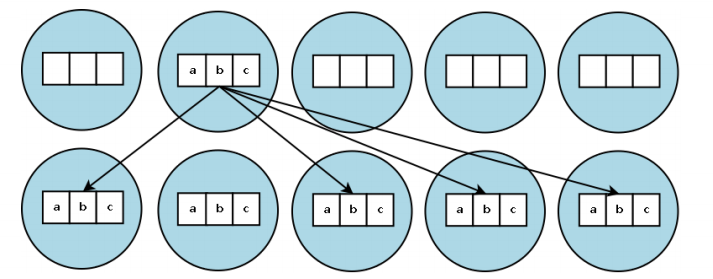
\includegraphics[width=\linewidth]{s1_int_broadcast.png}
\end{figure}

Operacja \texttt{\textbf{MPI\_Scatter}} polega na rozesłaniu przez proces root wektora sendbuf podzielonego na kawałki sendcount do procesów w grupie (również do siebie):
\begin{figure}[H]
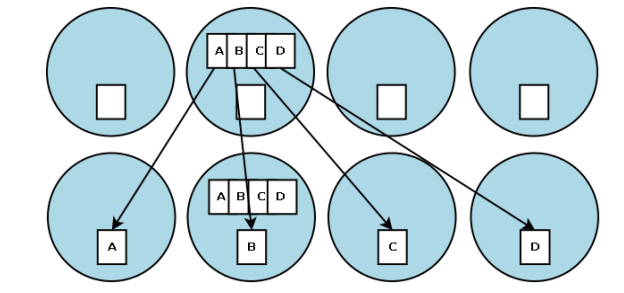
\includegraphics[width=\linewidth]{s1_int_scatter.png}
\end{figure}

Operacja \texttt{\textbf{MPI\_Gather}} odwrotna do scatter, czyli zebranie kawałków wektora z procesorów w grupie i zapisanie ich w buforze wybranego procesora.
\begin{figure}[H]
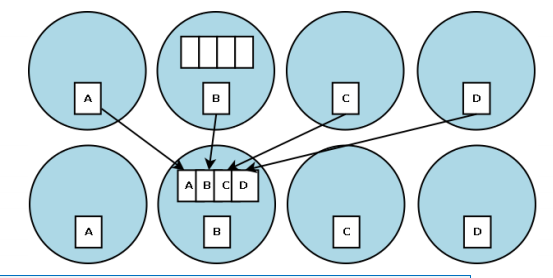
\includegraphics[width=\linewidth]{s1_int_gather.png}
\end{figure}

Operacja \texttt{\textbf{MPI\_AllGather}} jest analogiczna do \texttt{\textbf{MPI\_Gather}} z tą różnicą, że wynik jest umieszczany w \texttt{\textbf{recv\_buff}} każdego procesu. Można tą funkcję traktować jako ciąg kolejnych wywołań \texttt{\textbf{MPI\_Gather}} każdorazowo z innym numerem procesu \textbf{root}
\begin{figure}[H]
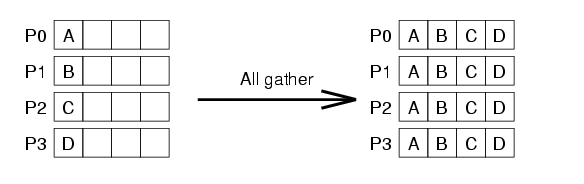
\includegraphics[width=\linewidth]{s1_int_allgather.png}
\end{figure}

Operacja wszyscy do wszystkich (\texttt{\textbf{MPI\_Alltoall}}). Każdy z procesów wysyła do procesu i-tego sendcount kolejnych elementów typu sendtype, poczynając od elementu i*sendtype tablicy sendbuf.
 
Operacja redukcji (\texttt{\textbf{MPI\_Reduce}}) służy do wykonywania globalnej operacji na elementach procesów należących do grupy. Pozwala wykonać na przykład sumowanie wszystkich częściowych wyników otrzymanych w procesach i umieszczenie wyniku w zmiennej. Przykładowe operatory to \textbf{MPI\_MAX}, \texttt{\textbf{MPI\_MIN}}, \texttt{\textbf{MPI\_SUM}} - kompletna lista znajduje się w dokumentacji. Istnieje również możliwość definiowania własnych operatorów dla funkcji \texttt{\textbf{MPI\_Reduce()}}.Warto wspomnieć o funkcji \textbf{MPI\_AllReduce}. Funkcja identyczna z poprzednią, różniąca się jedynie tym, że po jej wykonaniu wynik agregacji z użyciem operatora \textbf{op} znajduje się w zmiennej \textbf{result} we \underline{wszystkich} procesach.
